\documentclass[11pt,fleqn]{article}
\usepackage{array,multirow,amsthm,amsmath,amssymb,url}
% \usepackage[osf,sc]{mathpazo}
% Helvetica for sans serif
% (scaled to match size of Palatino)
% \usepackage[scaled=0.90]{helvet}
% Bera Mono for monospaced
% (scaled to match size of Palatino)
% \usepackage[scaled=0.85]{beramono}
% \usepackage{fullpage}
\newcommand{\RA}{\vdash}
\usepackage{mVersion}
\usepackage{natbib}
\usepackage{bussproofs}
\usepackage{tikz}
\usepackage{tikz-cd}
\usetikzlibrary{trees}
\title{First-order logic in syntactic approach}
\author{Hans Halvorson}
\date{\today}
% \setlength{\parindent}{0em}
% \setlength{\parskip}{1em}
\swapnumbers
\newtheorem{prop}{Proposition}
\newtheorem{thm}[prop]{Theorem}
\newtheorem{cor}[prop]{Corollary}
\newtheorem{lemma}[prop]{Lemma}
\newtheorem{claim}[prop]{Claim}
\newtheorem{fact}[prop]{Fact}
\newtheorem*{subthm}{Substitution Theorem}
\newtheorem*{rthm}{Replacement Theorem}
\newtheorem{conj}[prop]{Conjecture}
\theoremstyle{definition}
\newtheorem*{defn}{Definition}
\newtheorem{exercise}[prop]{Exercise}
\newtheorem*{example}{Example}
\theoremstyle{remark}
\newtheorem*{note}{Note}
\newtheorem*{disc}{Discussion}
\swapnumbers


% \usepackage{fbb}
\newcommand{\df}[1]{\textbf{#1}}
\usepackage{mathrsfs}
\newcommand{\2}{\mathscr}
\renewcommand{\emph}{\textbf}
\newcommand{\vp}{\varphi}

\usepackage[framemethod=TikZ]{mdframed}
\newcounter{axi}\setcounter{axi}{0}
\renewcommand{\theaxi}{\arabic{axi}}
\newenvironment{axi}[2][]{%
    \refstepcounter{axi}
 \ifstrempty{#1}%
% if condition (without title)
{\mdfsetup{%
    frametitle={%
        \tikz[baseline=(current bounding box.east),outer sep=0pt]
        \node[anchor=east,rectangle,fill=blue!20]
        {\strut Definition};}
    }%
% else condition (with title)
}{\mdfsetup{%
    frametitle={%
        \tikz[baseline=(current bounding box.east),outer sep=0pt]
        \node[anchor=east,rectangle,fill=blue!20]
        {\strut Definition};}%
    }%
}%
% Both conditions
\mdfsetup{%
    skipabove=2em,
    skipbelow=2em,
    innertopmargin=10pt,linecolor=blue!20,%
    linewidth=2pt,topline=true,%
    frametitleaboveskip=\dimexpr-\ht\strutbox\relax%
}
\begin{mdframed}[]\relax}{%
\end{mdframed}}

\begin{document}

\maketitle

First-order logic has pride of place in our best account of the
structure of knowledge.  In fact, there is reason to believe that
first-order logic is fully sufficient to encode all deductively valid
reasoning in mathematics, hence all deductively valid reasoning in the
mathematically rigorous empirical sciences.  It was discovered in the
early 20th century that first-order logic is powerful enough to
axiomatize many of the theories that mathematicians use, such as
number theory, group theory, ring theory, field theory, etc..  And
although there are other mathematical theories that are overtly
second-order (e.g.\ the theory of topological spaces quantifies over
subsets, and not just individual points), nonetheless first-order
logic can be used to axiomatize set-theory, and any second-order
theory can be formalized within set theory.  Thus, first-order logic
provides an expansive framework in which much, if not all, deductively
valid human reasoning can be represented.

Philosophers in the 20th century spent some time debating the question
of whether first-order logic is powerful enough to represent all such
valid reasoning.  We will return to that question in Chapter ??.  In
this chapter, we will study the properties of first-order logic, the
theories that can be formulated within it, and the relations that hold
between them.

Let's work from the ground up, beginning with a specific theory.

\begin{example}[The theory of partial orders] We suppose that there is
  a relation, which we'll denote by $\leq$, and we then proceed to lay
  down some postulates for this relation.  In particular:
\begin{itemize}
\item Postulate 1: The relation $\leq$ is reflexive in the sense that
  it holds between anything and itself.  For example, if we were
  working with numbers, we could write $2\leq 2$, or more generally,
  we could write $n\leq n$ for any $n$.  For this last phrase, we have
  a shorthand: we abbreviate it by $\forall n(n\leq n)$, which can be
  read out as, ``for all $n$, $n\leq n$.''  The symbol $\forall$ is
  called the \textbf{universal quantifier}.
\item Postulate 2: The relation $\leq$  is transitive in the sense
  that if $x\leq y$ and $y\leq z$, then $x\leq z$.  Again, we can
  abbreviate this last sentence as
  \[ \forall x\forall y\forall z((x\leq y\wedge y\leq z)\to x\leq z)
    ,\]
  which can be read as, ``for all $x$, for all $y$, and for all $z$,
  if \dots ''
  \item Postulate 3: The relation $\leq$ is asymmetric in the sense
    that if $x\leq y$ and $y\leq x$, then $x=y$.  This postulate can
    be formalized as:
    \[ \forall x\forall y((x\leq y\wedge y\leq x)\to x=y) .\]
  \end{itemize}
  In these previous postulates, we see the same logical connectives
  that we used in propositional logic, such as $\wedge$ and $\to$.
  But now these connectives might hold between things that are not
  themselves sentences.  For example, $x\leq y$ is not itself a
  sentence, because $x$ and $y$ aren't names of things.  We say that
  $x$ and $y$ are \textbf{variables}, and we say that $\leq$ is a
  \textbf{relation symbol}.  Finally, the familiar symbol $=$ is also
  a relation symbol. \hfill \qed \end{example}

We've described just the barest of bones of the theory of a partial
order.  There are a couple of further things that we would definitely
like to be able to do with this theory.  First, we would like to be
able to derive consequences from the postulates --- i.e.\ we would
like to derive theorems from the axioms.  In order to do so, we will
need to specify the \textbf{rules of derivation} for first-order
logic.  Second, we would like to be able to identify mathematical
structures that exemplify the axioms of partial order.  To do so, we
need to specify the \textbf{semantics}, or \textbf{model theory}, for
first-order logic.

%% Perhaps a couple more examples at this point?  e.g. mereology?
%% e.g. group theory

\begin{example}[The theory of abelian groups] We're all familiar with
  number systems such as the integers, the rational numbers, and the
  real numbers.  What do these number systems have in common?  One
  common structure between them is that they have a binary relation
  $+$, a neutral element $0$, and each number has a unique inverse.
  We also notice that the binary relation $+$ is associative in the
  sense that $x+(y+z)=(x+y)+z$, for all $x,y,z$.  We can formalize
  this last statement as
  \[ \forall x\forall y\forall z(x+(y+z)=(x+y)+z) .\]
  In these cases, the operation $+$ is also commutative, that is
  \[ \forall x\forall y(x+y=y+x ) .\] Bringing these postulates
  together, we have the theory of abelian groups.  Notice that in this
  case, we've enlarged our vocabulary to include a symbol $+$ and a
  symbol $0$.  The symbol $+$ is not exactly a relation symbol, but
  instead is a function symbol.  Intuitively speaking, given any names
  $n$ and $m$ of numbers, $n+m$ also names a number.  Similarly, $0$
  is taken to be the name of some specific number, and in this sense
  it differs from variables. \hfill \qed 
\end{example}

Abstracting from the previous examples, and many others like them
throughout mathematics, we now define the language of first-order
logic as follows.

\begin{defn} The \textbf{logical vocabulary} consists of the symbols
  $\bot,\forall ,\exists ,\wedge ,\vee ,\neg ,\to ,(, )$.  The symbol
  $\bot$ will serve as a propositional constant.  The final two
  symbols here are simply punctuation symbols that will allow us to
  keep track of groupings of the other symbols. \end{defn}

Please note that we intentionally excluded the equality symbol $=$
from the list of logical vocabulary.  Several philosophers in the 20th
century discussed the question of whether the axioms for equality were
``analytic truths,'' or whether they should count as part of a
contingent, non-logical theory.  We will not enter into that
discussion here.  Nonetheless, it will be helpful on a purely
technical level to treat the axioms for equality as a particular
theory.  We will also be taking a somewhat non-standard approach by
treating variables $x_1,x_2,\dots $ as part of the ``non-logical
vocabulary'' of a theory.  Our reason for doing so will become clear
when we discuss the notion of translations between theories.

\begin{defn} A \textbf{signature} $\Sigma$ consists of:
  \begin{enumerate} \item A countably infinite collection of
    \textbf{variables}.
  \item A collection of \textbf{relation symbols}, each of which is
    assigned a natural number called its \textbf{arity}.
  \item A collection of \textbf{function symbols}, each of which is assigned a
    natural number called its arity.
  \item A collection of \textbf{constant symbols}.  Note: constant
    symbols can also be considered as function symbols of zero
    arity. \end{enumerate}
\end{defn}

Some logicians use the name \emph{similarity type} as a synonym for
\emph{signature}.  There is also a tendency among philosophers to
think of a signature as an \emph{uninterpreted language}.  The idea
here is that the elements of the signature are symbols that receive
meaning by means of a semantic interpretation.

Although a list of variables is technically part of a signature, we
will frequently omit mention of the variables, and defer to using the
standard list $x,y,x_1,x_2,\dots $.  Only in cases where we are
comparing two theories will we need to carefully distinguish their
variables from each other.

\begin{example} For the theory of abelian groups, we used a signature
  $\Sigma$ that has a binary function symbol $+$ and a constant symbol
  $0$.  Some other presentations of the theory of abelian groups use a
  signature $\Sigma '$ that also has a unary function symbol ``$-$''
  for the inverse of an element.  Still other presentations of the
  theory use a signature that doesn't have the constant symbol $0$.
  We will discuss in Chapter ?? the sense in which these different
  theories all share the right to be called \textit{the} theory of
  abelian groups.  \hfill \qed \end{example}

\begin{disc} Let $\Sigma$ be the signature consisting of a binary
  relation symbol $r$, and let $\Sigma '$ be the signature consisting
  of a binary relation symbol $R$.  Are these signatures the same or
  different?  That depends on what implicit background conventions
  that we adopt, in particular, whether our specification of a
  signature is case-sensitive or not.  In fact, we could adopt a
  convention that was even more strict in how it individuates
  signatures.  For example, let $\Sigma ''$ be the signature
  consisting of a binary relation symbol $r$.  One could say that
  $\Sigma ''$ is a different signature from $\Sigma$ because the $r$
  in $\Sigma ''$ occurs at a different location on the page than the
  $r$ that occurs in $\Sigma$.  Of course, we would typically assume
  that $\Sigma =\Sigma '$, but such a claim depends on an implicit
  background assumption that there is a single letter form of which
  the two occurences of $r$ are instances.

  We will generally leave these implicit background assumptions
  unmentioned.  Indeed, to make these background assumptions explicit,
  we would have to rely on further implicit background assumptions,
  and we would never make progress in our study of first-order
  logic. \hfill \qed
\end{disc}

In Chapter ?? we will show a precise sense in which each first-order
theory is \textbf{equivalent} to a theory in a signature that has only
relation symbols (i.e.\ no function symbols or constant symbols).
Anticipating that result, we will first study the case of first order
theories that use only relation symbols, e.g.\ the theory of a partial
order.

\section*{Formation rules}

In this section, we suppose that $\Sigma$ is a fixed signature that
has no function or constant symbols.  (As we will see in Chapter ??,
there is a sense in which this assumption results in no loss of
generality.)  Since there are no function symbols, the definition of
\textbf{terms} is quite simple:

\begin{defn} A symbol $t$ is called a \textbf{term} of $\Sigma$ just
  in case $t$ is a variable $x$.  In this case, the variable $x$ is
  free in $t$.  \end{defn}

We shall now give an inductive definition that simultaneously defines
the notion of a \textbf{formula}, and of the \textbf{free variables}
in that formula.

\begin{defn} Let $\Sigma$ be a signature that consists of only
  relation symbols.  We define the set of \textbf{$\Sigma$-formulas}
  as follows:
\begin{enumerate}
\item $\bot$ is a formula that contains no free variables.
\item If $r$ is an $n$-ary relation symbol in $\Sigma$, and
  $t_1,\dots ,t_n$ are terms, then $r(t_1,\dots ,t_n)$ is a formula
  whose free variables are the union of all free variables in
  $t_1,\dots ,t_n$.
\item If $\phi$ and $\psi$ are formulas, then $\phi\wedge \psi$ is a
  formula whose free variables are the union of the free variables in
  $\phi$ and $\psi$.  Similarly for the other Boolean connectives
  $\neg ,\vee,\to$.
\item If $\vp$ is a formula, then so are $\exists x\vp$ and
  $\forall x\vp$.  The free variables in $\exists x\vp$ and
  $\forall x\vp$ are those in $\vp$, except possibly for $x$.  In
  other words, $\exists x\vp$ and $\forall x\vp$ contain no free
  occurrences of $\vp$, even if $\vp$ does.  \end{enumerate} We say
that a formula $\vp$ is \emph{closed}, or is a \emph{sentence}, if it
contains no free variables.  \end{defn}

As usual, a more fully precise definition of $\Sigma$-formulas would
make liberal use of parentheses.  For example, we would want to say
that $(\vp\wedge \psi )$ is a $\Sigma$-formula when $\vp$ and $\psi$
are $\Sigma$-formulas.  Nonetheless, we will continue to allow
ourselves to omit parentheses when no confusion is likely to result.

\begin{note} Our definition of the set of formulas allows for
  redundant quantification.  For example, the string
  $\exists x\forall x(x=x)$ is well-formed formula according to our
  definition.  This formula results from applying the quantifier
  $\exists x$ to the sentence $\forall x(x=x)$.  We will have to be
  careful in our definition of derivation rules, and semantic rules,
  to take the case of empty quantification into account.
\end{note}

%% Parse Tree?

It is helpful to think of formulas in terms of their \textbf{parse
  trees.}  For example, the formula
$\forall x\exists y(r(x,x)\to r(x,y))$ has the following parse tree:

\bigskip 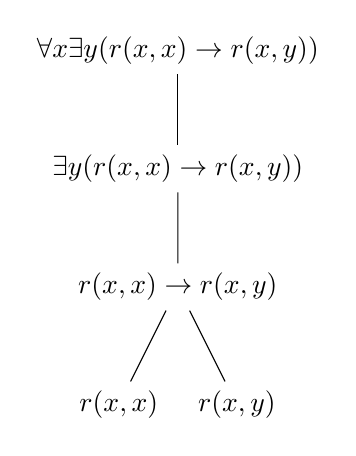
\begin{tikzpicture}[level distance=1.5cm,
  level 1/.style={sibling distance=3cm},
  level 2/.style={sibling distance=1.5cm}]
  \node {$\forall x\exists y(r(x,x)\to r(x,y))$}
    child {node {$\exists y(r(x,x)\to r(x,y))$}
      child {node {$r(x,x)\to r(x,y)$}
        child {node {$r(x,x)$}}
        child {node {$r(x,y)$}}}};
\end{tikzpicture}

\noindent The bottom nodes must each be elementary formulas, i.e.\
either $\bot$, or a relation symbol followed by the appropriate number
of variables.  Each parent-child relationship in the tree corresponds
to one of the Boolean connectives or to one of the quantifiers.

Formulas stand in one-to-one correspondence with parse trees: each
well-formed tree ends with a specific formula, and no other tree
yields the same formula.\footnote{Of course, we are not being fully
  explicit here about the identity conditions of parse trees.}  Using
the identity of formulas and parse trees, we can easily define a few
further helpful notions:

\begin{defn} Let $\vp$ be a $\Sigma$-formula.  The family of
  \textbf{subformulas} of $\vp$ consists of all those formulas that
  occur at some node in its parse tree.  \end{defn}

\begin{defn} If a quantifier $\exists x$ occurs in the formula $\vp$,
  then the \textbf{scope} of that occurrence is the formula which
  occurs at the immediately previous node in the parse
  tree.  \end{defn}

For example, in the formula $\forall x\exists y(r(x,x)\to r(x,y))$,
the scope of $\exists y$ is the formula $r(x,x)\to r(x,y)$.  In
contrast, in the formula $\forall x(r(x,x)\to \exists yr(x,y))$, the
scope of $\exists y$ is the formula $r(x,y)$.

We can now make the notion of free and bound variables even more
precise.  In particular, each individual occurrence of a variable in
$\vp$ is either free or bound.  For example, in the formula
$p(x)\wedge \exists p(x)$, $x$ occurs freely in the first subformula,
and bound in the second subformula.

\begin{defn}[Free and bound occurrences] An occurence of a variable
  $x$ in $\vp$ is \textbf{bound} just in case that occurrence is
  within the scope of either $\forall x$ or $\exists x$.  Otherwise
  that occurence of $x$ is free. \end{defn}

We could now perform a sanity check to make sure that our two notions
of bound/free variables coincide with each other.

\begin{fact} A variable $x$ is free in $\vp$ (in the sense of the
  definition of $\Sigma$-formulas) if and only if there is a free
  occurence of $x$ in $\vp$ (in the sense that this occurence does not
  lie in the scope of any corresponding quantifier).  \end{fact}

\begin{defn} We say that $y$ is free for $x$ in $\vp$ just in case no
  free occurrence of $x$ in $\vp$ is in the scope of the quantifier
  $\exists y$.  \end{defn}

Intuitively speaking, $y$ is free for $x$ just in case subtituting $y$
for $x$ does not result in $y$ being captured by $\exists y$ or
$\forall y$.  For example, in the formula $p(x)$, the variable $y$ is
free for $x$ (since $y$ is free in $p(y)$).  In contrast, in the
formula $\exists yp(x)$, the variable $y$ is not free for $x$ (since
$y$ is not free in $\exists yp(y)$).  We will need this notion in
order to formulate sound derivation rules.  For example, the rule of
$\forall$-elim should say something like:
$\forall x\vp (x)\vdash \vp (y)$.  However, if this rule were not
restricted in some way, then it would yield
\[ \forall x\exists y(x\neq y) \: \vdash \: \exists y(y\neq y) ,\]
which is clearly not valid.

It is also sometimes necessary to distinguish particular occurrences
of a subformula of a formula, and to define the \textbf{depth} at
which such an instance occurs.

\begin{defn} Let $\psi$ be a node in the parse tree of $\vp$.  The
  \textbf{depth} of $\psi$ is the number of steps from $\psi$ to the
  root node.  We say that $\psi$ is a \textbf{proper subformula} of
  $\vp$ if $\psi$ occurs with depth greater than $0$. \end{defn}

The parse trees of formulas are finite, by definition.  Therefore, the
depth of every occurrence of a subformula of $\vp$ is some finite
number.

There are a number of other properties of formulas that are definable
in purely syntactic terms.  For example, we could define the
\textbf{length} of a formula.  We could then note that the connectives
take formulas of a certain length and combine them to create formulas
of a certain greater length.

\begin{exercise} Show that no $\Sigma$-formula can occur as a proper
  subformula of itself. \end{exercise}



%% Example proofs by induction on construction?

Any time we define a set inductively, we have a corresponding method
of proof by induction.  In this case, we can prove that a property
$\mathbb{P}$ holds for all $\Sigma$-formulas by showing that
$\mathbb{P}$ holds for all elementary $\Sigma$-formulas, and that
$\mathbb{P}$ is preserved by the various operations that allow us to
construct more complex $\Sigma$-formulas.  What is a bit more
difficult in this case is proving that some property holds of all
$\Sigma$-sentences, when that property does not hold of all
$\Sigma$-formulas.  In such cases, we'll have to look for a clever way
to modify the standard sort of proof by induction.







\section*{Derivation rules}

We suppose again that $\Sigma$ is a fixed signature that has no
function or constant symbols.  We could then use any one of a myriad
of systems of derivation rules (axiomatic, natural deduction, sequent
calculus) to define the family of provable $\Sigma$-formulas.  These
rules will include analogues of the rules we provided for
propositional logic, and also some specific rules for introducing and
eliminating quantifiers.  For example, one might say that a
universally quantified sentence $\forall x\phi (x)$ implies any
instance $\phi (a)$; and that an instance $\phi (a)$ implies
$\forall x\phi (x)$ only if $\phi (a)$ was derived from something in
which the name ``$a$'' does not occur.  There are various ways that
these rule can be formulated, but there is widespread consensus on
what should be the extension of the provability relation $\vdash$
between sentences in first-order logic.  We will adopt the following
set of rules:

\begin{enumerate}
\item The rules for the Boolean connectives that we put forward in our
  discussion of propositional logic.  In this case, we permit
  derivations between formulas with free variables.  For example, we
  take
    \[ \vp (x)\wedge \psi (y) \: \vdash \: \vp (x) ,\] to be licensed
    by the rule of $\wedge$-elim.
  \item $\vp\wedge \neg p\:\vdash \: \bot$, for any formula $\vp$.
  \item $\bot \: \vdash \: \vp$, for any formula $\vp$.
  \item $\forall x\vp (x)\: \vdash \: \vp (t)$, where $t$ is any term
    that is free for $x$.
  \item $\vp \: \vdash $
\end{enumerate}



Although there are different ways we could specify the quantifier
rules, we will always have the following two results:
  \begin{enumerate}
  \item[(E1)] If $\vp\vdash \psi$, and $x$ does not occur free in
    $\psi$, then $\exists x\vp \vdash \psi$.
  \item[(E2)] If $\exists x\vp \vdash \psi$ then $\vp\vdash\psi$.
\end{enumerate}

We will make use of these facts in the proof of completeness in
Section ??.


\begin{defn} For formulas $\vp$ and $\psi$, we say that $\vp$ and
  $\psi$ are \emph{logically equivalent}, written $\vp\simeq\psi$,
  just in case both $\vp\vdash\psi$ and $\psi\vdash\vp$.
\end{defn}

The definition of $\simeq$ is patently symmetric.  The rule of
assumptions $\varphi\vdash\varphi$ entails that $\simeq$ is reflexive,
and the transitivity of $\vdash$ entails that $\simeq$ is transitive.
Thus, $\simeq$ is an equivalence relation on the set of
$\Sigma$-formulas.  Note that formulas $\vp$ and $\psi$ can be
equivalent in this sense even if they don't share all free variables
in common --- as long as the non-matching variables occur vacuously.
For example, $p(x)$ is equivalent to $p(x)\wedge (y=y)$, and it's also
equivalent to $p(x)\vee (y\neq y)$.  [The issue here has nothing in
particular to do with the equality relation.  The variable $y$ also
occurs vacuously in $p(y)\vee \neg p(y)$.]  In contrast, the formulas
$p(x)$ and $p(y)$ are not equivalent (in the empty theory), since it's
not universally valid that
$\vdash \forall x\forall y(p(x)\leftrightarrow p(y))$.

\begin{lemma} The relation $\simeq$ is compatible with the Boolean
  connectives in the following sense: if $\phi\simeq\phi '$ and
  $\psi\simeq \psi '$, then
  $(\phi\wedge \psi )\simeq (\phi '\wedge \psi ')$, and similarly for
  the other connectives. \end{lemma}

The proof of this lemma is straightforward if you know the
introduction and elimination rules for the Boolean connectives.


%% Deduction theorem?

%% Sufficient sets of connectives

%% TO DO: Does it also work with the quantifiers?  Careful, could
%% capture a free variable in one of the formulas


\section*{Translation and substitution}

Suppose that $\Sigma$ and $\Sigma '$ are predicate logic signatures.
At this point, we are working with single-sorted logic, which means
that $\Sigma$ is a list of relation symbols, function symbols, and
constant symbols.  Similary for $\Sigma '$.  Suppose now that we are
looking for a way to translate formulas of $\Sigma$ to formulas of
$\Sigma '$.  As usual, we begin by assigning the elements of the
signature $\Sigma $ to syntactic objects built from $\Sigma '$.  Now,
you might initially think that a relation symbol $r\in \Sigma$ ought
to be assigned to some corresponding relation symbol in $\Sigma '$.
But recall the case of propositional logic.  In that case, we found it
convenient sometimes to translate an elementary sentence, such as $p$,
to a complex sentence in another language.  The only important thing
was that sentences should be mapped to sentences.

Similarly, a \textbf{reconstrual} of $\Sigma$ into $\Sigma '$ will
assign each relation symbol $r$ of $\Sigma$ to some corresponding open
formula $r_F$ of $\Sigma '$.  For example, suppose that $r$ is a
binary relation symbol in $\Sigma$, and that $\Sigma '$ has two unary
relation symbols $p$ and $q$.  Then, for example, $r(x,y)$ could be
reconstrued as the open formula $p(x)\wedge \neg q(y)$.  Similarly, if
$\Sigma '$ contains a ternary relation symbol $s$, then $r(x,y)$ could
be reconstrued as the open formula $\exists z\,s(x,y,z)$.

Note that, in both cases, we reconstrued $r(x,y)$ as a formula $r_F$
of $\Sigma '$ that shares the same free variables as $r$.  That
assumption should strike you as a little bit suspicious.  Why think
that the language built on $\Sigma $ should share exactly the same
variables as the language built on $\Sigma '$?  (And your answer
shouldn't be: that's how we did it in my introduction to logic class.)
It's not like variables have some ``trans-theoretical'' meaning that
must be preserved by any reasonable translation.

But how then can variables be reconstrued in moving from one theory to
another?  One natural proposal would be to include in a reconstrual a
mapping from variables of $\Sigma$ to variables of $\Sigma '$, i.e.\ a
function that assigns a variable of $\Sigma '$ to each variable of
$\Sigma$.  Even so, it's a non-trivial question whether there is an
in-principle reason that a single variable in $\Sigma$ must be
reconstrued as a single variable in $\Sigma '$.  Perhaps one theorist
uses several variables to do the work that the other theorist manages
to do with a single variable.  Such cases are not hard to find in the
sciences --- for example, when the objects of one mathematical theory
are reconstrued as ``logical constructions'' of objects in another
mathematical theory.

\begin{enumerate}
\item In the 19th century, the German mathematician Leopold Kronecker
  is reported to have said, ``God made the integers, all else is the
  work of man.''  In more prosaic terms, talk about higher number
  systems --- such as rational, real, and complex numbers --- can be
  reduced to talk about integers.  However, to effect such a
  reduction, one must treat each rational number as a pair of integers
  --- or, more accurately, as an equivalence class of pairs of
  integers.  Similarly, to reduce the complex numbers to the real
  numbers, one must treat a complex number as a pair of real numbers,
  viz.\ the real and imaginary parts of the complex number.
\item Now for a more controversial example, which we will take up at
  greater length in Chapter ??.  There are different ways that one can
  write down axioms for Euclidean geometry.  In one axiomatization,
  the basic objects are points; and in another axiomatization, the
  basic objects are lines.  Is there a sense in which these two
  axiomatized theories could both be Euclidean geometry, in
  particular, that they could be equivalent?  The answer is Yes, but
  only if one allows translations that take a single variable of the
  first theory to a pair of variables of the second theory.  In
  particular, a line needs to be treated as an equivalence class of
  pairs of points; and a point needs to be treated as a pair of
  intersecting lines.
  \end{enumerate}

  Let's proceed then under the assumption that a single variable in
  one language could be reconstrued in terms of multiple variables in
  another language.  Thus, a \textbf{reconstrual}, in the formal
  sense, should include a function that matches variables of the
  signature $\Sigma$ to $n$-tuples of variables of the signature
  $\Sigma'$.  For simplicity, we will often indicate such a map by
  using primed variables.  For example, a variable $x$ is mapped to
  $x'_1,\dots ,x'_n$.  But recall that such a map is not given in
  advance --- giving a translation includes specifying some particular
  map.

  So far we have: a reconstrual $F$ assigns relation symbols to open
  formulas, and variables to $n$-tuples of variables.  There are still
  a couple more pieces of data that we wish to include in a
  reconstrual.

  First of all, consider again the case of reconstruing rational
  numbers (i.e.\ fractions) as pairs of integers.  Of course, not
  \emph{every} pair of integers gives a well-defined fraction.  For
  example, there is no fraction of the form $\frac{1}{0}$.  In that
  case, the ``integer theorist'' doesn't think of the domain of
  fractions as consisting of all pairs of integers; rather, she thinks
  of that domain as consisting of pairs of integers where the second
  entry is non-zero.

  To capture this nuance --- the restriction of the domain of
  quantification --- we stipulate the a reconstrual $F$ includes a
  formula $u_F$ of the target language $\Sigma '$.  In the running
  example, the formula $u_F$ could be given by
  \[ u_F(x,y) \: \equiv \: (x=x)\wedge (y\neq 0) .\] The integer
  theorist can then use the formula $u_F$ to restrict her quantifiers
  to the domain of well-defined fractions.

  Finally, and perhaps most controversially, let's consider how we
  might reconstrue the equality relation $=$ of the domain theory $T$
  as a relation of the target theory $T'$.  Recall that the single
  variables $x$ and $y$ will typically be reconstrued as $n$-tuples of
  variables $\vec{x}$ and $\vec{y}$.  In that case, how should we
  reconstrue the formula $x=y$?  One might naturally propose that
  $x=y$ be reconstrued as the formula
  \begin{equation} (x_1=y_1)\wedge (x_2=y_2)\wedge \cdots \wedge
    (x_n=y_n) .\label{simple} \end{equation} But here we need to think
  a bit harder about how and why variables of $\Sigma$ are encoded as
  variables of $\Sigma '$.  For this, let's consider again the example
  of rational numbers being reduced to integers.

  \begin{example} Consider a formula $x=y$ in the theory of rational
    numbers.  To the ``integer theorist,'' the variables $x$ and $y$
    really represent complex entities, namely fractions.  What's more,
    to say that two fractions $\frac{x_1}{x_2}$ and $\frac{y_1}{y_2}$
    are equal does not mean that $x_1=y_1$ and $x_2=y_2$.  Rather,
    $\frac{x_1}{x_2}=\frac{y_1}{y_2}$ means that
    $x_1\times y_2=y_1\times x_2$.  In other words, the formula $x=y$
    of the language of the rational numbers is reconstrued as the
    formula
    \begin{equation} x_1\times y_2=y_1\times x_2
      ,\label{foo} \end{equation} in the language of the integers,
    where $\times$ is the multiplication operation. \hfill
    \qed \end{example}

  This example suggests that we might not always want the formula
  $x=y$ to be reconstrued as Eqn.\ \ref{simple}.  Instead, we might
  prefer to reconstrue $x=y$ as some other $\Sigma '$ formula
  $e(x_1,\dots ,x_n;y_1,\dots ,y_n)$.  Of course, not everything goes:
  $e$ will need to perform the same functions in the theory $T'$ that
  the formula $x=y$ performs in the theory $T$.  In particular, we
  will require that $e$ is an equivalence relation relative to the
  theory $T'$.

  We're now ready to propose a general definition of a translation
  between predicate logic theories.  We begin with the notion of a
  \textbf{reconstrual}, which provides a dictionary matching elements
  of the signature $\Sigma$ with syntactic objects built from
  $\Sigma '$.  \def\vp{\varphi}

\begin{axi}{} Let $\Sigma$ and $\Sigma '$ be single-sorted predicate
    logic signatures.  An \textbf{$n$-dimensional reconstrual} $F$ of
    $\Sigma$ into $\Sigma '$ consists of:
    \begin{enumerate}
    \item A mapping of variables of $\Sigma$ to $n$-tuples of distinct
      variables of $\Sigma '$.  For simplicity, we will often suppress
      any explicit mention of this mapping, and rely instead on
      suggestive notation --- e.g.\ using $x_1,\dots ,x_n$ or
      $\vec{x}$ for the $n$-tuple corresponding to $x$.  We also
      require that if $x$ and $y$ are distinct variables of $\Sigma$,
      then $\vec{x}$ and $\vec{y}$ are non-overlapping $n$-tuples of
      variables of $\Sigma '$.
    \item An $n$-ary formula $u_F(\vec{x})$ of $\Sigma$, picking out
      the target domain of the reconstrual.
    \item A $2n$-ary formula $e_F(\vec{x},\vec{y})$ of $\Sigma '$,
      picking out the intended interpretation of the equality relation
      for $\Sigma$.
    \item For each $m$-ary relation symbol $r$ of $\Sigma$, an
      $mn$-ary formula $r_F$ of $\Sigma '$.  (To be fully precise, we
      would need to specify which variables occur in $r_F$.  On an
      intuitive level, a unary relation $r(x)$ will correspond to an
      $n$-ary relation $r_F (x_1,\dots ,x_n)$, where $x_1,\dots ,x_n$
      are the variables assigned by the reconstrual to $x$.)
    \end{enumerate}
  \end{axi}

  As we now show, a reconstrual $F$ of $\Sigma$ into $\Sigma '$
  naturally extends to a map from $\Sigma$-formulas to
  $\Sigma '$-formulas.  If $\vp$ is a $\Sigma$-formula, we will
  typically use $\vp _F$ to designate the corresponding $\Sigma '$
  formula.  

  \begin{itemize}
  \item An elementary formula $r(x)$ of $\Sigma$ is assigned to the
    formula $r_F(\vec{x})$ of $\Sigma '$.  (Notice here the use of the
    mapping between the variable $x$ of $\Sigma$ and the $n$-tuple
    $\vec{x}$ of variables of $\Sigma '$.)
  \item The elementary formula $x=y$ of $\Sigma$ is assigned to the
    formula $e_F(\vec{x},\vec{y})$ of $\Sigma '$.
  \item Extending recursively, define
    \[ (\phi\wedge \psi )_F \: = \: \phi _F\wedge \psi _F ,\]
    and similarly for the other Boolean connectives. 
  \item Extending recursively, define
  \[ (\exists x \phi (x))_F \: \equiv \: \exists
    \vec{x}(u_F(\vec{x})\wedge \phi _F ) .\] 
  and
  \[ (\forall x\phi (x))_F\:\equiv \: \forall \vec{x}(u_F(\vec{x})\to \phi
    _F ) .\]
\end{itemize}
The quantifier clauses of this definition could use some
clarification.  Roughly speaking, the quantifier $\exists x$ is
translated as $\exists x_1\cdots \exists x_n$, relativized to the
domain $u_F$.  Similarly, $\forall x$ is translated as
$\forall x_1\cdots \forall x_n$, again relativized to the domain
$u_F$.  Keep in mind, however, that the meaning of the resulting
quantifiers $\exists x_1\cdots \exists x_n$ and
$\forall x_1\cdots \forall x_n$ also depends on the corresponding
equality relation, which in this case is $e_F$.

\begin{thm} If $F$ is a reconstrual and $\vp\vdash\psi$ then
  $\vp _F\vdash \psi _F$. \end{thm}

\begin{proof} We will prove this result by induction on the definition
  of the relation $\vdash$.  For the base case, the rule of
  assumptions justifies not only $\vp\vdash\vp$, but also
  $\vp _F\vdash\vp _F$.  The inductive cases for the Boolean
  connectives involve no special complications, and so we omit them.

  Consider then the case of $\exists$-elim.  Suppose that
  $\exists x\vp (x)\vdash \psi$ results from $\vp (x)\vdash \psi$,
  where $x$ is not free in $\psi$.  The inductive hypothesis here says
  that $(\vp (x))_F\vdash \psi _F$, which can be rewritten as
  $\vp _F(\vec{x})\vdash \psi _F$.  We need to show that
  $(\exists x\vp (x))_F\vdash \psi _F$, which can be rewritten as
  \[ \exists \vec{x}(u_F(\vec{x})\wedge \vp _F(\vec{x}))\vdash \psi _F \]

\end{proof}






%% substitution -- see Belnap, maybe Kleene  

  \begin{defn} Let $\phi$ be a $\Sigma$-formula, and let $x$ and $y$ be
  variables.  We will use the notation $\phi (y/x)$ to denote the
  result of a ``safe substitution'' of $y$ for all free occurrences of
  $x$ in $\phi$.  By ``safe substitution,'' we mean to prohibit cases
  where a free occurrence of $x$ would become a bound occurrence of
  $y$.  For example, in the formula $\exists y\, r(x,y)$, replacing
  $x$ with $y$ would result in the new variable $y$ becoming captured.
  Such can be prevented by choosing a variable $z$ that does not occur
  in $\phi$, replacing occurrences of $\exists y$ with $\exists z$,
  and corresponding bound occurrences of $y$ with $z$, then replacing
  all free occurences of $x$ with $y$.
\end{defn}

%% seems that I need to know that \phi (y/x) is equivalent to \phi

%% Step 1: alpha equivalence -- this is easy

%% Step 2: replacement by equivalent subformulas -- this is hard? yes,
%% a little bit

\subsection*{Replacement}

Intuitively speaking, it seems obvious that if a subformula $A$ of
$\vp _A$ is replaced with an equivalent subformula $B$, then the
resulting formula $\vp _B$ will be equivalent to the original.  Here
we will state the result more precisely, and sketch its proof.

When we say that $A$ and $B$ are \textbf{logically equivalent}, we
simply mean that $\vdash A\leftrightarrow B$.  Or, if using a proof
system that applies only to closed sentences, then we say that $A$ and
$B$ are logically equivalent just in case
\[ \vdash \forall x_1\cdots \forall x_n(A\leftrightarrow B) , \] where
$x_1,\dots ,x_n$ is the list of variables with free occurrences in
either $A$ or in $B$.  

The key lemmas for proving replacement are Lemma ?? and the following:

\begin{lemma} If $A(x)\simeq B(x)$ then
  $\exists xA(x)\simeq \exists xB(x)$. \end{lemma}

\begin{proof}[Sketch of proof] Given $A(x)\simeq B(x)$, we have
  $\vdash A(x)\to B(x)$, and hence $\vdash A(x)\to \exists xB(x)$ by
  $\exists$-intro.  Since $x$ does not occur free in $\exists x B(x)$,
  it follows that $\vdash \exists xA(x)\to \exists xB(x)$ by
  $\exists$-elim.  A similar argument shows that
  $\vdash \exists x B(x) \to \exists x A(x)$.  Therefore
  $\exists x A(x)\simeq \exists x B(x)$. \end{proof}
  
\begin{rthm} Suppose that $\vp _B$ is the formula that results from
  replacing $A$ in $\vp _A$ with $B$.  If $A\simeq B$ then $\vp
  _A\simeq \vp _B$. 
\end{rthm}



\section*{{\S}  The syntactic view of theories}

%% Observation and theoretical vocabulary
%% Putnam, Achinstein, van Fraassen critique



\end{document}
